\chapter{Motivația și formularea problemei}

\section*{Contextul general și relevanța problemei}

Expresiile faciale constituie canalul principal al comunicării afective nonverbale, jucând un rol fundamental în interacțiunea socială umană \cite{sariyanidi2015}. Sistemele informatice convenționale, însă, interacționează cu utilizatorii aproape exclusiv prin conținut verbal sau textual, ignorând în mare măsură această dimensiune esențială a comunicării.

Deficitul devine critic în contextele în care persoana nu poate sau nu dorește să verbalizeze starea afectivă:
\begin{itemize}
	\item Pacienții cu boli neurodegenerative (demență, Alzheimer);
	\item Persoanele cu tulburări din spectrul autist;
	\item Pacienții sedați sau postoperator;
	\item Copiii mici sau persoanele care nu vorbesc limba personalului medical.
\end{itemize}

În toate aceste situații, un sistem capabil să detecteze automat și în timp real stările emoționale exclusiv pe baza expresiei faciale ar constitui un instrument clinic de valoare considerabilă, permițând personalului medical să reacționeze prompt la semnale de disconfort, durere sau anxietate care altfel ar trece neobservate.

Dincolo de contextul clinic, aplicațiile recunoașterii automate a emoțiilor faciale (\textit{Facial Emotion Recognition} - FER) acoperă un spectru larg: monitorizarea atenției șoferilor, sisteme de tutoriat inteligent, analize de marketing și interfețe om-calculator adaptive pentru realitate virtuală.

\section*{Formularea problemei}

Problema abordată în prezenta lucrare poate fi enunțată formal astfel: dat fiind un flux video al feței unui subiect uman, să se construiască un sistem automat care mapează fiecare secvență de cadre la una dintre cele șapte categorii emoționale fundamentale definite în modelul extins al lui Ekman \cite{ekman1986new, ekman1992argument}: \textit{Anger, Contempt, Disgust, Fear, Happiness, Sadness} și \textit{Surprise}.

\begin{description}
	\item[Intrarea sistemului:] O secvență de cadre video (în cazul de față, câte $10$ cadre extrase din setul de date CK+), care surprind evoluția temporală a expresiei faciale de la starea neutră până la apexul emoției. 
	\item[Ieșirea sistemului:] Un vector de probabilități al emoțiilor. În cadrul aplicației \textbf{Neuro-Guardian}, aceste date sunt agregate temporal pentru calculul scorurilor de \textit{suferință} și \textit{durere}.
\end{description}

Procesul intern investigat în cazul rețelelor neuronale bazate pe spike-uri (SNN) este descris printr-un pipeline structurat în cinci etape principale, ilustrat schematic în Figura~\ref{fig:pipeline_general}. Acesta se parcurge secvențial de la stânga la dreapta și începe cu etapa de \textbf{Input Video}, în care datele brute formate din secvențe video grayscale ($48 \times 48$ pixeli, 10 cadre/secv.) sunt introduse în sistem. În faza de \textbf{Preprocesare}, se realizează configurarea setului de date prin împărțirea în pliuri de antrenare și testare (\textit{Train+Test sequences}) și selectarea unui algoritm de eșantionare (\textit{Random, Landmark, BoundingBox} sau \textit{OnOffSaliency}). Urmează \textbf{Codificare Spikes}, etapă în care imaginile sunt transformate în reprezentări temporale sub formă de trenuri de impulsuri ($t \in [0.0, 1.0]$) prin tehnici precum filtre \textit{On/Off} și \textit{Latency Coding}. Ulterior, modulul \textbf{CSNN 3D} extrage trăsăturile spațio-temporale utilizând convoluții 3D bazate pe învățare nesupervizată de tip STDP, inhibiție și homeostazie. În urma decodificării, hărțile de caracteristici trec printr-un mecanism de pooling \textit{spațial} și \textit{temporal}. În final, în etapa \textbf{SVM $\rightarrow$ Emoție}, clasificatorul analizează vectorul de trăsături rezultat pentru a determina distribuția probabilistică a celor șapte emoții țintă și a stabili eticheta finală dominantă.

\begin{figure}[htbp]
	\centering
	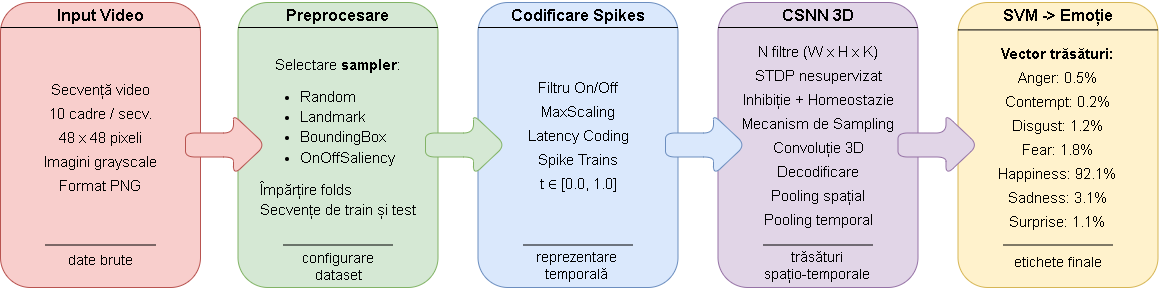
\includegraphics[width=0.99\textwidth]{figures/pipeline.drawio.png} 
	\caption{Schema bloc a sistemului propus: de la fluxul video la clasificarea emoțiilor prin SNN.}
	\label{fig:pipeline_general}
\end{figure}

\section*{Dificultatea recunoașterii emoțiilor}

Deși recunoașterea expresiilor faciale (FER) partajează cu recunoașterea obiectelor statice provocări fundamentale, precum similitudinea inter-clasă în plan static (unde elemente vizuale comune pot genera confuzii macro), specificul FER aduce o complexitate majoră determinată de natura sa intrinsec dinamică. În mod particular, FER se confruntă cu o variabilitate intra-clasă ridicată, întrucât aceeași emoție se poate manifesta prin tipare de mișcare și intensități faciale extrem de diverse de la un individ la altul. La această dificultate specifică se adaugă problema generică a dezechilibrului de clase din seturile de date academice (precum CK+), unde o distribuție neuniformă a eșantioanelor afectează direct capacitatea de generalizare în timpul antrenării. Mai mult, eficiența procesării secvențiale a fluxului video devine un criteriu critic pentru sistem; constrângerile impuse de o aplicație în timp real (precum Neuro-Guardian) cer o latență redusă per cadru, ceea ce limitează utilizarea modelelor \textit{deep learning} masive și impune soluții optimizate pentru analiza temporală. 

Deși arhitecturile clasice (CNN-LSTM) ating acuratețe ridicată (de $88.37\%$ în cadrul experimentelor realizate și descrise în Secțiunea \ref{sc:cnn-lstm}), ele implică un cost energetic substanțial prin înmulțiri matriciale continue. 

Rețelele neuronale cu impulsuri adresează această ineficiență prin:
\begin{enumerate}[noitemsep]
	\item \textbf{Activare bazată pe evenimente:} Neuronii consumă energie doar atunci când generează un \textit{spike}. În perioadele de imobilitate facială, activitatea rețelei este minimă.
	\item \textbf{Filtrarea naturală a zgomotului:} Prin filtrarea On/Off, pixelii statici din fundal nu generează impulsuri, concentrând calculul exclusiv pe zonele cu dinamică relevantă.
	\item \textbf{Codificarea temporală (\textit{Latency Coding}):} Trăsăturile proeminente produc impulsuri timpurii, creând o ierarhie temporală pe care regula STDP o exploatează pentru a învăța trăsături spațio-temporale fără a avea nevoie de etichete în faza de antrenare.
\end{enumerate}

\section*{Încadrarea în literatura de specialitate}
%\addcontentsline{toc}{chapter}{Încadrarea în literatura de specialitate}

\subsection*{Recunoașterea emoțiilor faciale folosind rețele SNN bio-inspirate}

Lucrarea elaborată de Mansouri-Benssassi și Ye \cite{mansouri2021} investighează aplicabilitatea rețelelor neuronale cu impulsuri (SNN) bio-inspirate în sarcini de recunoaștere a emoțiilor faciale (FER), punând un accent deosebit pe robustețea la zgomot și capacitatea de generalizare. Arhitectura propusă adaptează modelul Diehl și Cook \cite{diehl2015}, utilizând învățarea nesupervizată prin plasticitate dependentă de timpul impulsurilor (STDP). Procesarea imaginilor implică utilizarea filtrului Laplacian of Gaussian (LoG) pentru extracția eficientă a marginilor, urmată de o codificare de tip \textit{rate coding} prin trenuri de impulsuri Poisson, unde intensitatea pixelilor dictează rata de declanșare a neuronilor de tip Leaky Integrate-and-Fire (LIF). Modelul este structurat pe trei straturi: unul de intrare, un strat excitator (cu funcții de convoluție) și un strat inhibitor pentru selecția neuronului activ. Evaluările realizate pe seturile de date JAFFE și CK+ relevă faptul că SNN-ul obține performanțe comparabile cu metodele HOG+SVM și superioare arhitecturilor CNN pe seturi de date mici. Un aspect critic evidențiat este superioritatea SNN în experimentele de generalizare \textit{cross-dataset} (atingând până la 92\%) și reziliența remarcabilă la zgomot de tip \textit{salt and pepper}; la un nivel de degradare de 0,5, SNN menține o acuratețe de 56,2\%, depășind net modelele CNN (22,6\%) și SVM (14,1\%). Totuși, se identifică limitări privind utilizarea codificării pe bază de rată în detrimentul celei temporale și necesitatea rulării pe hardware neuromorfic dedicat pentru a maximiza eficiența energetică și computațională față de implementările actuale pe CPU/GPU.

\subsection*{Abordări bazate pe evenimente: Arhitectura Spiking-FER}

O contribuție majoră în domeniu este adusă de Barchid et al. \cite{barchid2023}, care introduc conceptul de „Event-based FER” și propun primul benchmark de acest tip prin conversia seturilor de date video clasice (CK+, ADFES, CASIA și MMI) în fluxuri de evenimente folosind simulatorul V2E \cite{yuhuang2021}. Autorii propun \textit{Spiking-FER}, o arhitectură SNN convoluțională profundă bazată pe SEW-ResNet-18, care utilizează neuroni de tip \textit{Integrate-and-Fire} (IF). Pentru a permite antrenarea de tip \textit{end-to-end} și a depăși problema non-diferențiabilității funcției de prag, se utilizează \textit{Surrogate Gradient Learning} cu o aproximare bazată pe funcția arctan. Spre deosebire de metodele modulare, abordarea \textit{end-to-end} permite optimizarea simultană a extractorului de trăsături și a clasificatorului. Rezultatele experimentale indică faptul că \textit{Spiking-FER} atinge performanțe comparabile cu modelele ANN, însă cu o eficiență energetică net superioară, fiind de până la 65,39 ori mai eficient din punct de vedere computațional. Studiul analizează, de asemenea, impactul tehnicilor de augmentare a datelor specifice evenimentelor (\textit{Event Data Augmentation}), concluzionând că metodele \textit{EventDrop} și \textit{Mirror} sunt esențiale pentru reglarea antrenării pe seturi de date limitate. Totuși, o limitare importantă a studiului rămâne dependența de date simulate în locul senzorilor DVS (\textit{Dynamic Vision Sensor}) reali și utilizarea bazelor de date de laborator, care pot să nu reflecte complexitatea emoțiilor spontane din mediul real.

\subsection*{Recunoașterea emoțiilor prin senzori de viziune dinamică simulați}

Într-o direcție asemănătoare, lucrarea propusă de Wang et al. \cite{wang2022} abordează deficitul de seturi de date pentru senzori de viziune dinamică (DVS) în recunoașterea emoțiilor prin propunerea unei metode de generare a datelor simulate din segmente video convenționale (setul CMU-MOSI \cite{zadeh2016}). Autorii introduc un cadru SNN bazat pe modelul de neuron \textit{Parametric Leaky Integrate-and-Fire} (PLIF), care permite optimizarea automată a parametrilor de scurgere (\textit{leak}) în timpul antrenării. O contribuție metodologică importantă este utilizarea unei prime rame de tip \textit{float-value} pentru a stabiliza potențialul de membrană, urmată de trenuri de impulsuri binare, strategie care accelerează scăderea funcției de pierdere și îmbunătățește a\-cu\-ra\-te\-țea față de modelele care folosesc exclusiv \textit{spikes}. Arhitectura este compusă dintr-un modul de extracție a trăsăturilor cu straturi convoluționale și \textit{average pooling}, un grup de neuroni de votare și un modul de mapare emoțională care traduce ratele de declanșare în etichete de polaritate. Antrenarea se realizează prin gradient surogat și \textit{backpropagation through time} (BPTT). Rezultatele experimentale demonstrează că modelul SNN reduce consumul de energie cu 75\% față de echivalentul ANN, atingând performanțe optime la un prag de tensiune de 0,4. Totuși, datele simulate nu pot reproduce fidel rezoluția temporală fină a unui senzor DVS real, iar constrângerea ferestrei temporale la 68 de cadre poate duce la pierderea informațiilor în cazul secvențelor video de lungimi inegale.

\subsection*{Fuziunea multimodală și arhitecturi evolutive: Modelul FusionSense}

Lucrarea prezentată de Tan et al. \cite{tan2020} introduce \textit{FusionSense}, primul sistem de recunoaștere a emoțiilor bazat pe rețele neuronale cu impulsuri care utilizează fuziunea datelor multimodale (expresii faciale corelate cu semnale fiziologice precum ECG, conductanța pielii și respirația). Autorii utilizează cadrul \textit{NeuCube} \cite{kasabov2014}, o arhitectură SNN evolutivă (eSNN) care încorporează o structură spațială 3D de tip \textit{reservoir} (3D-SNNr) cu conectivitate \textit{small-world}. Pipeline-ul vizual utilizează algoritmul Viola-Jones pentru detecție și metoda Kanade-Lucas-Tomasi (KLT) pentru urmărirea punctelor de interes, extrăgând distanțe relative între 68 de repere faciale (\textit{landmarks}) raportate la o stare neutră de referință. Un aspect metodologic distinct este utilizarea codificării de tip \textit{population coding} bazată pe câmpuri receptive Gaussiene, urmată de o învățare nesupervizată prin STDP și o etapă supervizată ce folosește reguli de tip \textit{Rank Order} (deSNN). Experimentele pe setul de date MAHNOB-HCI demonstrează că fuziunea la nivel de trăsături (\textit{feature-level fusion}) este superioară celei la nivel de decizie, atingând o acuratețe de 73,15\% pentru valența binară. Sistemul se remarcă prin capacitatea de antrenare incrementală (\textit{one-pass}), fiind optim pentru aplicații \textit{real-time}. Totuși, studiul prezintă limitări legate de excluderea semnalelor EEG și de dependența de o fereastră temporală fixă de 30 de secunde, care poate omite dinamica emoțională pe termen lung.

\subsection*{Recunoașterea identității prin dinamica mișcărilor faciale}

Lucrarea propusă de Liu et al. \cite{liu2020} introduce o paradigmă inovatoare de re\-cu\-noaș\-te\-re facială bazată pe dinamica mișcărilor musculare, metodă eficientă chiar și în scenarii cu fețe deghizate sau parțial ocultate. Spre deosebire de sistemele convenționale care se bazează pe trăsături spațiale statice, acest model utilizează cadre diferențiale pentru a captura micro-mișcările unice induse de vorbire. Arhitectura este de tip SNN profund, structurată pe cinci straturi care simulează calea ventrală a sistemului vizual biologic, incluzând module de extracție a trăsăturilor de nivel înalt prin filtre Gabor și codificare temporală bazată pe \textit{Rank Order Coding} (ROC). Un element central al modelului este stratul de învățare care utilizează mecanismul \textit{Soft Winner-Take-All} (WTA) cu inhibiție laterală și reguli STDP \textit{event-driven}, asigurând selectivitatea neuronilor pentru tipare motorii specifice. Evaluările pe setul de date MakeFaceDB au demonstrat rate de succes între 95\% și 100\%, depășind modelele CNN echivalente, în special în scenariile cu deghizări complexe (măști, barbă falsă). Autorii subliniază eficiența procesului de convergență, care necesită doar două clipuri video pentru antrenare. Totuși, sunt identificate limitări practice importante: dependența de mișcarea activă a subiectului (necesitatea de a vorbi), sensibilitatea ridicată la mișcările de fundal sau ale camerei și necesitatea unei reglări manuale riguroase a hiperparametrilor pentru a menține stabilitatea rețelei.

\subsection*{Concluzii}
Capitolul de față a stabilit cadrul general al lucrării: necesitatea clinică a unui sistem automat de recunoaștere a emoțiilor faciale, formularea formală a problemei ca mapare a secvențelor video la cele șapte categorii emoționale fundamentale ale modelului Ekman, și principalele dificultăți tehnice --- variabilitatea intra-clasă ridicată, similaritatea inter-clasă, dezechilibrul de clase și constrângerile de eficiență computațională în timp real. Totodată, analiza literaturii de specialitate a evidențiat că rețelele neuronale cu impulsuri reprezintă o direcție promițătoare, capabilă să depășească metodele clasice în scenarii de generalizare cross-dataset și de robustețe la zgomot, cu un potențial semnificativ de eficiență energetică pe hardware neuromorfic dedicat. Pornind de la aceste premise, capitolul următor prezintă fundamentele teoretice necesare înțelegerii arhitecturii propuse: tranziția de la modelele SVM, la ANN clasice și până la SNN, modelarea matematică a neuronului cu impulsuri, filtrele On/Off, schemele de codificare neurală și mecanismele de plasticitate sinaptică pe care se bazează întregul pipeline experimental, arhitecturile CSNN, metode de eșantionare și de decodificare a impulsurilor.